\documentclass[tikz]{standalone}
\begin{document}
    \usetikzlibrary{shapes,arrows,positioning,automata}
    \usetikzlibrary{matrix,arrows,decorations.pathmorphing}
    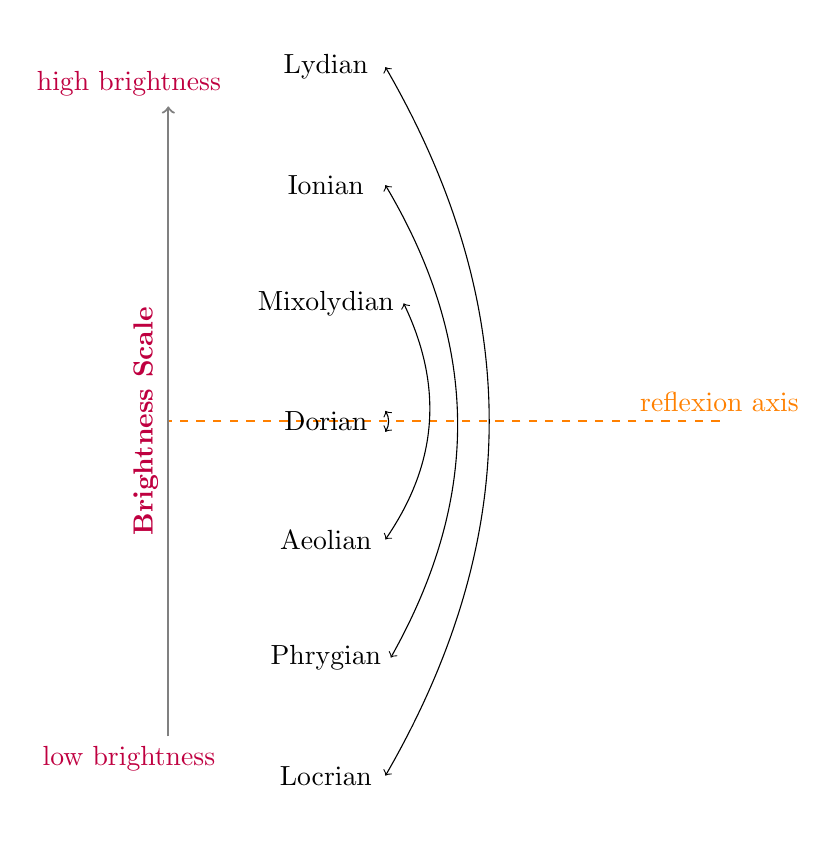
\begin{tikzpicture}[
        auto,
        node distance=1.5cm,
        block/.style={color=black, align=center, minimum height=1cm, minimum width=1.5cm},
        vec/.style={thick,color=black!50}
      ]
      \draw[thick,dashed,color=orange] (5, 0) -- (-2, 0) node[above,color=orange] at (5, 0) {reflexion axis};
      \node[block,] at (0, 0) (dor)   {\normalsize Dorian};
      \node[block,above of=dor] (mix) {\normalsize Mixolydian};
      \node[block,above of=mix] (ion) {\normalsize Ionian};
      \node[block,above of=ion] (lyd) {\normalsize Lydian};
      \node[block,below of=dor] (aeo) {\normalsize Aeolian};
      \node[block,below of=aeo] (phr) {\normalsize Phrygian};
      \node[block,below of=phr] (loc) {\normalsize Locrian};
      \draw[vec,->] (-2, -4) -- (-2, 4)
        node[above,sloped,color=purple] at (-2.5, 4) {high brightness}
        node[midway,above,sloped,color=purple] at (-2.5, 0) {\textbf{Brightness Scale}}
        node[below,sloped,color=purple] at (-2.5, -4) {low brightness};
      
      \path[<->]   (lyd.east) edge [bend left=30] (loc.east);
      \path[<->]   (ion.east) edge [bend left=30] (phr.east);
      \path[<->]   (mix.east) edge [bend left=30] (aeo.east);
      \path[<->]   (dor.10) edge [bend left=30] (dor.350);
      
      % \draw (ion.east) to node[auto, swap] {} (phr.east);
      % \draw (mix.east) to node[auto, swap] {} (aeo.east);
      % \draw[bend left=90] (dor.30) to node[auto, swap] {} (dor.330);
    \end{tikzpicture}
\end{document} 
